\documentclass{beamer}
\mode<presentation>
\usepackage{amsmath}
\usepackage{amssymb}
\usepackage{adjustbox}
\usepackage{subcaption}
\usepackage{enumitem}
\usepackage{multicol}
\usepackage{mathtools}
\usepackage{listings}
\usepackage{url}
\usepackage{circuitikz}
\def\UrlBreaks{\do\/\do-}
\usetheme{Boadilla}
\usecolortheme{seahorse}
\setbeamertemplate{footline}
{
  \leavevmode%
  \hbox{%
  \begin{beamercolorbox}[wd=\paperwidth,ht=2.25ex,dp=1ex,right]{author in head/foot}%
    \insertframenumber{} / \inserttotalframenumber\hspace*{2ex} 
  \end{beamercolorbox}}%
  \vskip0pt%
}
\setbeamertemplate{navigation symbols}{}

\providecommand{\nCr}[2]{\,^{#1}C_{#2}} % nCr
\providecommand{\nPr}[2]{\,^{#1}P_{#2}} % nPr
\providecommand{\mbf}{\mathbf}
\providecommand{\pr}[1]{\ensuremath{\Pr\left(#1\right)}}
\providecommand{\qfunc}[1]{\ensuremath{Q\left(#1\right)}}
\providecommand{\sbrak}[1]{\ensuremath{{}\left[#1\right]}}
\providecommand{\brak}[1]{\ensuremath{\left(#1\right)}}
\providecommand{\cbrak}[1]{\ensuremath{\left\{#1\right\}}}
\providecommand{\abs}[1]{\left\vert#1\right\vert}
\providecommand{\norm}[1]{\lVert#1\rVert}
\providecommand{\mtx}[1]{\mathbf{#1}}
\providecommand{\mean}[1]{E\left[ #1 \right]}
\providecommand{\fourier}{\overset{\mathcal{F}}{ \rightleftharpoons}}
\providecommand{\system}{\overset{\mathcal{H}}{ \longleftrightarrow}}
\providecommand{\dec}[2]{\ensuremath{\overset{#1}{\underset{#2}{\gtrless}}}}
\newcommand{\myvec}[1]{\ensuremath{\begin{pmatrix}#1\end{pmatrix}}}
\let\vec\mathbf

\lstset{
frame=single, 
breaklines=true,
columns=fullflexible
}

\numberwithin{equation}{section}

\title{Gradient Ascent}
\author{CHARAN RONGALI \\ Electrical Engineering,\\IIT Hyderabad}
\date{\today} 

\begin{document}

\begin{frame}
\titlepage
\end{frame}

\section*{Outline}
\begin{frame}
\tableofcontents
\end{frame}

\section{Problem Statement}
\begin{frame}
\frametitle{Problem Statement}
Show that the altitude of the right circular cone of maximum volume that can be inscribed in a sphere of radius $R$ is $\frac{4R}{3}$.
\end{frame}

\section{Solution}
\subsection{Geometric Analysis}
\begin{frame}
\frametitle{Geometric Analysis}

\begin{columns}
    \column{0.6\textwidth}
    Let $R$ be the radius of the sphere, and let $h$ be the height (altitude) of the inscribed cone. Let $x$ be the radius of the base of the cone.

    By considering a cross-section of the sphere and the inscribed cone, we relate $x$, $h$, and $R$ using the Pythagorean theorem. The center of the sphere lies on the axis of the cone.
    \begin{align}
        x^2 + (h-R)^2 &= R^2 \\
        x^2 + h^2 - 2hR + R^2 &= R^2 \\
        x^2 &= 2hR - h^2
    \end{align}

    \column{0.4\textwidth}
    \centering
    \begin{adjustbox}{max width=\textwidth}
        \begin{circuitikz}
        \tikzstyle{every node}=[font=\Large]
        \draw  (7.25,19) circle (5.5cm);
        \draw [short] (7.5,24.5) -- (2.5,16.25);
        \draw [short] (7.5,24.5) -- (12,16.25);
        \draw  (7.25,16.25) ellipse (4.75cm and 0.5cm);
        \draw [short] (7.5,16.25) -- (12,16.25);
        \draw [short] (7.5,24.5) -- (7.5,16.25);
        \draw [short] (7.5,19.25) -- (12,16.25);
        \node [font=\Large] at (9.75,18.5) {R};
        \node [font=\Large] at (6.25,17.5) {h - R};
        \node [font=\Large] at (9.25,16) {\textit{x}};
        \node [font=\Large] at (6.75,21.25) {R};
        \end{circuitikz}
    \end{adjustbox}

\end{columns}

\end{frame}

\subsection{Volume Maximization}
\begin{frame}
\frametitle{Volume Maximization}
The volume $V$ of the cone is given by:

\begin{align}
V &= \frac{1}{3} \pi x^2 h \\
V &= \frac{1}{3} \pi (2hR - h^2) h \\
	V &= \frac{1}{3} \pi (2Rh^2 - h^3)   \implies \sbrak{ Cost Function}
\end{align}

To maximize the volume, we take $\frac{dV}{dh} = 0$:
\begin{align}
\frac{dV}{dh} &= \frac{1}{3} \pi (4Rh - 3h^2) \\
0 &= h(4R - 3h) \implies h \neq 0\\
4R - 3h &= 0 \\
h &= \frac{4R}{3}
\end{align}
\end{frame}

\subsection{Second Derivative Test}
\begin{frame}
\frametitle{Second Derivative Test}
To confirm a maximum, we take the second derivative:

\begin{align}
\frac{d^2V}{dh^2} &= \frac{1}{3} \pi (4R - 6h)
\end{align}

Substituting $h = \frac{4R}{3}$:

\begin{align}
\frac{d^2V}{dh^2} &= \frac{1}{3} \pi (4R - 8R) \\
&= -\frac{4\pi R}{3}
\end{align}

Since this is negative, $h = \frac{4R}{3}$ gives a maximum volume.
\end{frame}

\subsection{Computational Approach}
\begin{frame}
\frametitle{Computational Approach}
Using Gradient Ascent, the update rule is:

\begin{align}
h_{n+1} &= h_n + \alpha \frac{dV}{dh} \Big|_{h=h_n}
\end{align}

For our case:

\begin{align}
h_{n+1} &= h_n + \alpha \frac{\pi}{3} (4Rh_n - 3h_n^2)
\end{align}

Choosing:

\begin{align}
R &= 1, \quad \alpha = 0.0001, \quad h_0 = 0.5
\end{align}

This converges to $h = \frac{4}{3}$.
\end{frame}

\subsection{Graphical Representation}
\begin{frame}
\frametitle{Graphical Representation}
After a few iterations, the value of $h$ will converge to approximately $\frac{4}{3} \approx 1.333$.
\begin{figure}[h]
\centering
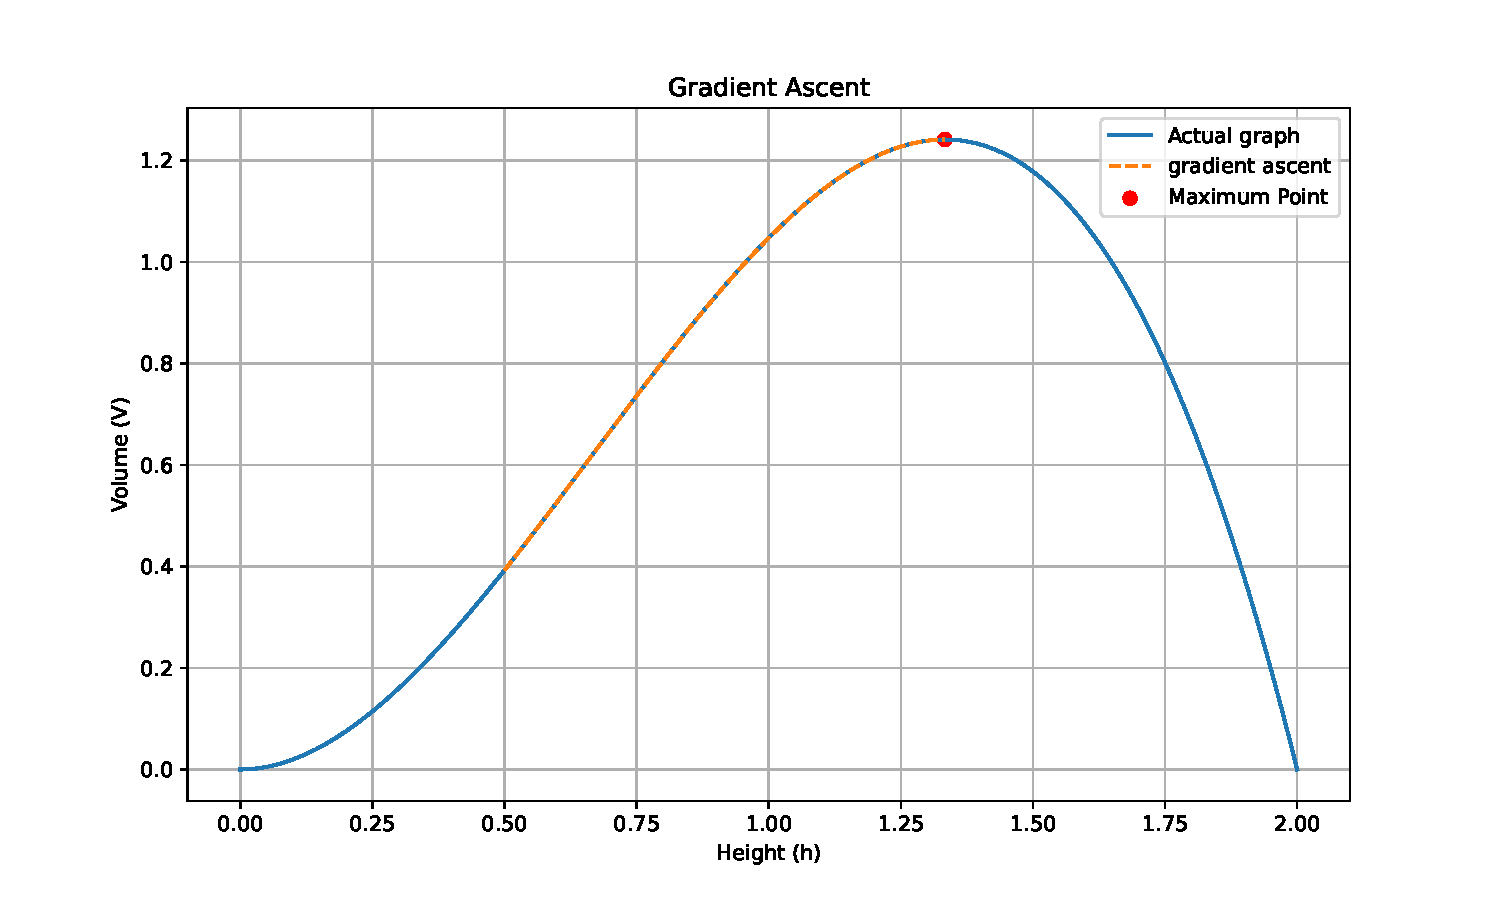
\includegraphics[width=0.9\linewidth]{figs/plot.pdf}
\end{figure}
\end{frame}

\end{document}

